
\chapter{The RepNet-MDP framework}
\label{chap:mdp}
The primary goal of this thesis is to study the properties of the RepNet framework. More concretely, the concepts of \textit{action distribution}, \textit{image}, \textit{reputation}, and \textit{directed actions}, as well as their impact on RepNet agents' behavior are key elements that distinguish it from classic (Partially Observable) Markov Decision Processes. While the notion of \textit{partial observability} for RepNet agents differs slightly from the definition employed by POMDP agents, in that RepNet agents have to keep track of the state in which other agents believe to be in addition to their own belief, it is arguably the feature that separates RepNet-POMDPs the least from other MDP-derived frameworks. In an attempt to bring the RepNet framework closer to \textit{tractability} and simplify the study of its properties, it can be reduced from its POMDP setting to a fully observable setting. Several adjustments, covered in \RefSec{sec:reduct}, are necessary to make the starting framework \textit{fully observable}. 
Further alleviation of the \textit{intractability} of the framework can be achieved by favoring approximate solutions of satisfactory quality over exact solutions. To this end, a look-ahead-based approach similar to that described in the context of classic MDPs in \RefSec{sec:stateart} can be taken.

This chapter follows the following structure: \RefSec{sec:reduct} describes the steps necessary to reduce the RepNet framework to a fully observable setting and follows with the presentation of the reduced framework. \RefSec{sec:reimagined} provides a solution to the concept of \textit{directed actions} imagined by \textit{Rens et al.} \cite{rensetal}. \RefSec{sec:revv} reviews the concept of \textit{action distribution estimation} in fully observable settings. \RefSec{sec:planningoptimal} then discusses planning for optimal impact in the context of RepNet-MDPs. \RefSec{sec:onlineplan} introduces the online look-ahead algorithm used to further alleviate the intractability of the reduced RepNet framework. Finally, \RefSec{sec:genn} briefly reviews the mathematical definition of \textit{reputation}.


%\section{Intractability of the RepNet-POMDP framework}
%\label{sec:intrapo}

\section{Reduction of the RepNet-POMDP framework}
\label{sec:reduct}
A RepNet-MDP is, analogously to its POMDP counterpart (\RefDef{def:name}), defined as a tuple
\begin{align*}
    \mathcal{M} := \big \langle \Sigma, \Gamma \big \rangle.
  \end{align*}
where $\Sigma$ is the \textit{system} tuple and $\Gamma$ is the \textit{agents} tuple. Several adjustments are necessary to make the starting framework fully observable. 
\begin{itemize}
    \item The system as defined in \RefDef{def:systempo} includes the set of possible observations $\Omega$. Given that neither impact function $\mathcal{I}$ nor update function $\mathcal{U}$ make use of $\Omega$, it may be removed without further ramifications in the new definition of the system (\RefDef{def:system}).
    \item The agents that make up $\Gamma$ in \RefDef{def:agentspo} notably each have their own observation function $O_g$, which furthermore appears in several equations: 
    \begin{enumerate}
        \item Each agent $g$'s subjective perception of the world is maintained in the functions $AD_g$, $Img_g$, and $B_g$. The update of these concepts is conditioned by the observations it makes.
        \item The optimality equations (\RefDef{def:optipo}) sum over all possible observations, after which the recursive calls to the value function are weighted using the observation function.
    \end{enumerate}
    In a fully observable environment, each agent is completely aware of the current state of the environment, rendering the belief state function $B_g$ of each agent $g$ futile. More specifically,
    \begin{enumerate}
        \item Each agent $g$'s image function $Img_g$ is updated partly on the basis of $g$'s current belief function, as it appears in the expected total impact function (\RefDef{def:imppo}).
        \item The perceived immediate impact on agent $g$ (\RefDef{def:perceivedpo}) is likewise conditioned by its current belief state function $B_g$, and is simplified in the reduced framework.
        \item The recursive calls in the optimality equations are weighted by the agent's current belief state function.
    \end{enumerate}
\end{itemize}

\begin{definition}[RepNet-MDP system]
\label{def:system}
A system in a RepNet-MDP $\Sigma$ is formally defined as a tuple
\begin{align*}
    \Sigma := \big \langle \mathcal{G}, \mathcal{S}, \mathcal{A}, \mathcal{I}, \mathcal{U} \big \rangle
  \end{align*}
where $\mathcal{G}$, $\mathcal{S}$, $\mathcal{A}$, $\mathcal{I}$, and $\mathcal{U}$ are defined as in \RefDef{def:systempo}.
\end{definition}

\begin{definition}[Agents]
\label{def:agents}
Let $\Gamma$ be a tuple embedding each agent's subjective understanding of the environment it operates in, such that
\begin{align*}
    \Gamma := \big \langle \{UT_g\}, \{DT_g\}, \{AD_g\}, \{Img_g\} \big \rangle
  \end{align*}
where $UT_g$, $DT_g$, $AD_g$, and $Img_g$ are defined as in \RefDef{def:agentspo}.
\end{definition}

The updated definition of \textit{expected total impact} is given in \RefDef{def:imp}, while its effect on the \textit{image function} is given in \RefDef{def:img}.
\begin{definition}[Expected total impact]
\label{def:imp}
According to agent $g$, the total impact an agent $h$ is expected to have on, as well as perceive from, another agent $i$, assumed to be different from $h$, when the environment is in state $s$, is defined as
\begin{align*}
    ETI_{g} (h, i, s, AD_g) :=  \sum_{a \in \mathcal{A}} \, \big[ \, \delta AD_g(i, s)(a) \mathcal{I}(h, i, s, a)  + (1 - \delta) AD_g(h, s)(a) \mathcal{I}(i, h, s, a) \, \big]
\end{align*}
where $\delta \in [0,1]$ trades off the relative importance of impact due to agent $h$ and impact perceived by $h$.
\end{definition}

\begin{definition}[Image update]
\label{def:img}
Let $Img_g$ be the current image function of agent $g$. The updated image function $Img_g'$ is computed as follows:
\begin{align*}
     Img_g' &:= IE(g,Img_g,\alpha, s, AD_g) \\&:= \Big\{(h,i, t) \,\,\Big| \,\,h,i \in \mathcal{G} \land t =  \mathcal{U}(\alpha, Img_g(h,i), ETI_{g}(h, i,s, AD_g)) \Big\}
\end{align*}
where
\begin{itemize}
    \item $IE$ is called the \textit{image estimation function}.
    \item $\alpha$ is called the learning rate.
    \item $s$ is the current state of the environment.
\end{itemize}
\end{definition}

The mathematical definition of reputation for RepNet-POMDPs (\RefDef{def:reppo}), given by
\begin{align}
    REP_g(h, Img_g) := \frac{1}{|\mathcal{G}|} \sum_{i \in \mathcal{G}} Img_g(h,i) \times Img_g(i,g),
\end{align}
can produce undesirable results in regards to self-reputation. To demonstrate this, consider a scenario in which two agents, say $A$ and $B$, are deployed in an environment without ever having been in contact with one another. Their image of each other can, therefore, be assumed neutral, i.e.,
\begin{align}
    Img_A(B, A) = 0, \,\,\,\,\,\,\,\, Img_A(B,A) = 0.
\end{align}
At this point, the desired reputation-related numbers should show that agent $A$ believes every agent's reputation, including its own, to be neutral. While this is indeed the case for agent $B$'s reputation, the same does not apply to agent $A$'s self-reputation. In fact,
\begin{align*}
\label{eq:selfrep2}
    REP_A(A, Img_A) &= \frac{1}{2} \,\, \big[ Img_A(A,B) \times Img_A(B,A) + Img_A(A,A) \times Img_A(A,A) \big]
    \\&= \frac{1}{2} \,\, \big[ 0 + 1\big] = \frac{1}{2}.
\end{align*}
As such, agent $A$ believes itself to initially have a higher reputation than agent $B$. The definition of reputation that follows was adjusted to address this inconvenience.


\begin{definition}[Adjusted Reputation]
\label{def:repnew}
The reputation of an agent $h$, according to agent $g$, is formally defined as 
\begin{align*}
      REP_g(h, Img_g) := 
    \begin{cases}
    \frac{1}{|\mathcal{G}|} \sum_{i \in \mathcal{G}} Img_g(h,i) \times Img_g(i,g) & \mbox{if } h \neq g
    \\
    \frac{1}{|\mathcal{G}|-1} \sum_{i \in \mathcal{G} \setminus \{ g \}} Img_g(h,i) \times Img_g(i,g) & \mbox{otherwise}
    \end{cases}
\end{align*}
where $Img_g(i,i) = 1 \,\,\forall i \in \mathcal{G}$.
\end{definition}





\section{Reimagined concept of directed actions}
\label{sec:reimagined}
In \RefSec{sec:dirr}, the concept of \textit{directed} transitions, as it was developed by \textit{Rens et al.} \cite{rensetal}, was covered. Using a trading example between two agents, of which the transition model of the environment $\mathcal{T}$ is repeated in \RefFig{fig:dir15}, two problems were identified.


\begin{figure}[h]
  \begin{center}
    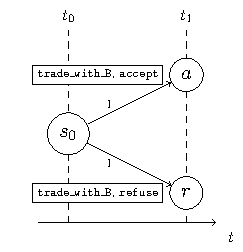
\includegraphics[width=0.4\textwidth]{images/MasterThesisDirectedActionsDraw (2).pdf}
  \end{center}
  \caption{Transition model $\mathcal{T}$ of the trading example. $s_0$ is the initial state, $a$ is the \textit{accept} state, and $r$ is the \textit{refuse} state. The transition model of the environment $\mathcal{T}$ is assumed to be deterministic.}\label{fig:dir15}
\end{figure}



The first problem resides in the fact that agent $A$ has not yet performed action \texttt{trade\_with\_B} at time $t_0$ and, as such, agent $B$ is not aware of $A$'s intentions. Concretely, there is no incentive for agent $B$ to favor action \texttt{accept} over action \texttt{refuse} at $t_0$. This problem is easily addressed by adding an \textit{intermediate} state $s_1$, in which agent $B$ is made aware of agent $A$'s desire to trade, to the transition model of the environment, and by rearranging the combinations of actions between any two states. The transition model with the intermediate state added is given in \RefFig{fig:dir2}.

\begin{figure}[h]
  \begin{center}
    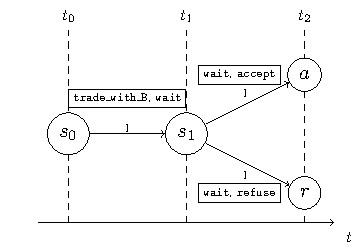
\includegraphics[width=0.6\textwidth]{images/MasterThesisDirectedNewDraw (2).pdf}
  \end{center}
  \caption{Updated transition model $\mathcal{T}$ of the trading example, $s_1$ is the state in which Agent $B$ is made aware of the trade offer.}\label{fig:dir2}
\end{figure}

The second problem pertains to the fact that \textit{directed} transition models can not describe the actual rules of the environment. In the case of the trade between agents $A$ and $B$, they can, at most, describe agent $A$'s \textit{subjective} impression of the impact that its own reputation might have on the willingness of agent $B$ to accept its trade offers. 
As such, one must make a clear distinction between the purpose of an \textit{undirected} transition model, which describes the actual rules of the environment as they apply to a single agent, and that of a \textit{directed} transition model, which describes that agent's \textit{subjective} perception of the rules of the environment. A version of the trading scenario between agents $A$ and $B$ that was adapted to make use of the concept of directed actions is presented hereafter.

The environment is made up of the same set of states $\mathcal{S} = \{s_0, s_1, a, r\}$ depicted in \RefFig{fig:dir2}. The set of \textit{undirected} actions at the disposal of both agents is given by
\begin{align}
    \mathcal{A}^u = \{\texttt{trade\_with\_B}, \texttt{accept}, \texttt{refuse}, \texttt{wait}\}.
\end{align}
\textit{In the eyes of} agent $A$, agent $B$'s response to a trade offer depends on $A$'s reputation. Concretely, $s_1 \rightarrow a$ and $s_1 \rightarrow r$
make up the transitions for which agent $A$ believes its reputation to be relevant. The action taken by agent $A$ during these transitions is \texttt{wait}. To make use of the notion of directed actions, the set of \textit{directed} actions $\mathcal{A}^d$ will contain the equivalent of \texttt{wait} in its \textit{directed} form, that is,
\begin{align}
    \mathcal{A}^d = \{\texttt{wait\_d}\}.
\end{align}

The way agent $A$ makes use of actions in $\mathcal{A}^u$ and $\mathcal{A}^d$ can now be detailed.
When reasoning about the value of each action, that is, when \textit{planning} to maximize its expected impact, agent $A$ will make use of \textit{undirected} actions in $\mathcal{A}^u$ whenever the action currently investigated has no equivalent in $\mathcal{A}^d$. For instance,
    \begin{align}
        T_A(A, s_0, \texttt{trade\_with\_B}, s_1, r_A) = UT(A, s_0, \texttt{trade\_with\_B}, s_1).
    \end{align}
    When an action in $\mathcal{A}^u$ has an equivalent in $\mathcal{A}^d$, agent $A$ will make use of the concept of directed actions in planning to maximize its expected impact. For instance,
    \begin{align}
        T_A(A, s_1, \texttt{wait}, a, r_A) = DT_A(A, s_1, \texttt{wait\_d}, a, r_A). 
    \end{align}
As such, the reputation of agent $A$ is accounted for when agent $A$ \textit{plans} to maximize its expected impact.
It is worth stressing that the rules of the environment do not change when agent $A$ reasons in terms of directed actions. Moreover, when agent $A$ is in $s_1$ and is to wait for agent $B$'s response to the trade offer, the action that is performed on the environment is the \textit{undirected} variant \texttt{wait}.










\section{Reviewing the action distribution estimation function}
\label{sec:revv}

The next step in the formalization of RepNet-MDPs consists in redefining the updating scheme of the action distribution $AD_g$ of each agent $g$. Initially, the reasoning applied here is similar to that applied to RepNet-POMDPs. Say an environment hosting two agents $g$ and $h$ is currently in state $s$. Agent $g$ has an \textit{a priori} notion of the probability of agent $h$ picking an action $a$ in state $s$,
\begin{align}
    P_g(a | h, s,r_h).
\end{align}
Following agent $h$ performing action $a$ in this state, the environment transitions from state $s$ to state $s'$. The \textit{a posteriori} probability of agent $h$ performing that same action $a$ in state $s$ in the future is now computed using Bayes' rule:
\begin{align}
\begin{split}
    P_g(a | h,s,r_h,s') &= \frac{P_g(s' | h,s,r_h,a) P_g(a | h, s,r_h)}{P_g(s'|h,s,r_h)} 
    \\
    &= \frac{P_g(s' | h,s,r_h,a) P_g(a | h, s)}{\sum_{a'} P_g(s'|h,s,r_h,a') P_g(a' | h,s)}.
\end{split}
\end{align}
The probabilities may now be replaced by the terms defined in \RefDef{def:agents} and \RefDef{def:globtran}:
\begin{align}
\label{eq:updateeq}
    AD_g'(h,s)(a) = \frac{T_g(h,s,a,s', r_h) AD_g(h,s)(a)}{\sum_{a'} T_g(h,s,a',s', r_h) AD_g(h,s)(a')}.
\end{align}




While MDP-derived formalisms are designed to deal with stochastic environments, one should expect them to work with deterministic transition models. The \textit{action distribution update} in \textit{fully observable} settings, as given in Equation \ref{eq:updateeq}, can produce undesirable results that make it impossible for a RepNet agent to \textit{unlearn} what it has learned.
Consider the trading scenario between agents $A$ and $B$ described in \RefSec{sec:reimagined} and whose transition model is schematized in \RefFig{fig:dir2}. The transitions of the environment are assumed to be deterministic, that is,
\begin{align}
    UT(B, s_1, \texttt{accept}, a) = 1, \,\,\,\,\, UT(B, s_1, \texttt{refuse}, r) = 1.
\end{align}
If agent $B$ refuses the trade offer made by agent $A$, the environment transitions to state $r$ and the action distribution is updated as follows:

\begin{align*}
    AD_A'(B,s_1)(\texttt{accept}) &=   \frac{UT(B,s_1, \texttt{accept},r) AD_A(B,s_1)(\texttt{accept})}{\sum_{a'} UT(B,s_1,a',r) AD_A(B,s_1)(a')}
    \\&=  \frac{0 \cdot AD_A(B,s_1)(\texttt{accept})}{\sum_{a'} UT(B,s_1,a',r) AD_A(B,s_1)(a')}
    \\&= 0
\end{align*}

\begin{align*}
    AD_A'(B,s_1)(\texttt{refuse}) &=   \frac{UT(B,s_1, \texttt{refuse},r) AD_A(B,s_1)(\texttt{refuse})}{\sum_{a'} UT(B,s_1,a',r) AD_A(B,s_1)(a')}
    \\&=  \frac{1 \cdot AD_A(B,s_1)(\texttt{refuse})}{\sum_{a'} UT(B,s_1,a',r) AD_A(B,s_1)(a')}
    \\&= 1
\end{align*}



As dictated by the new action distribution, agent $A$ is, in the wake of a \textit{single} unsuccessful trade, convinced that agent $B$ will never accept any trade offer in the future. Moreover, the primary issue does not reside in the fact that agent $A$ was quick to make up its mind, but in the fact that it is now impossible for agent $A$ to change its strategy in the future. In fact, the probability of $B$ accepting a trade is 0, and regardless of what this value is multiplied by in the future, it will always remain 0. 

This inconvenience is addressed hereafter by applying a \textit{smoothing} technique called \textit{Laplace smoothing} \cite{laplacesmoothing}. Let $\mathbf{\theta} = \langle \theta_1, \theta_2, ..., \theta_d \rangle$, such that $\theta_i \in [0,1] \,\, \forall i$ and $\sum_{i} \theta_i = 1$, be the probabilities of a multinomial distribution with $d$ categories. The \textit{Laplace-smoothed} estimators of the probabilities are given by

\begin{align}
    \hat{\theta}_i = \frac{\theta_i + \eta}{\sum_i (\theta_i + \eta)} = \frac{\theta_i + \eta}{\sum_i \theta_i + d\eta},
\end{align}
where $\eta \in [0,1]$ is called the \textit{smoothing parameter}. If $\theta_i \gg \eta$, then $\hat{\theta}_i \simeq \theta_i$. If $\theta_i \ll \eta$, then $\hat{\theta}_i \simeq \frac{1}{d}$. The smoothing technique thus prevents probabilities of 0 from ever occurring. The same smoothing technique can be applied to the \textit{action distribution update} function, resulting in the following equation:

\begin{align}
\label{eq:adu}
    AD_g'(h,s)(a) = \frac{T_g(h,s,a,s', r_h) AD_g(h,s)(a) + \eta}{\sum_{a'} (T_g(h,s,a',s', r_h) AD_g(h,s)(a') + \eta)}.
\end{align}

The new definition of the \textit{action distribution estimation} function (\RefDef{def:actupnew}) takes this smoothing technique into account.

\begin{definition} [Adjusted Action distribution update]
\label{def:actupnew}
Let $AD_g$ be the current action distribution function of agent $g$. The updated action distribution function $AD_g'$ is computed as follows:
\begin{align*}
     AD_g' &:= ADE(g, s', AD_g, Img_g) \\&:= \Bigg\{(h,s,a,p) \,\,\Bigg| \,\, h \in \mathcal{G} \land s \in \mathcal{S} \land a \in \mathcal{A} \,\land r_h = REP_g(h,Img_g)
     \\& \,\,\,\,\,\,\,\,\,\,\, \land p =  \frac{T_g(h,s,a,s', r_h) AD_g(h,s)(a) + \eta}{\sum_{a'} (T_g(h,s,a',s', r_h) AD_g(h,s)(a') + \eta)} \Bigg\}
\end{align*}
where
\begin{itemize}
    \item $ADE$ is called the \textit{action distribution estimation function}.
    \item $s'$ is the state the environment transitions to.
    \item $\eta$ is the \textit{smoothing parameter}.
\end{itemize}
\end{definition}













\section{Planning for optimal impact}
\label{sec:planningoptimal}

Optimal behavior in the context of RepNet-MDPs may now be described. To simplify the notation in this as well as in later sections, a construct called \textit{epistemic state} is defined hereafter.
\begin{definition}[Epistemic state]
\label{def:know}
The epistemic state $\theta_g$ of agent $g$ is formally defined as a tuple
\begin{align*}
     \theta_g := \big \langle s,  AD_g, Img_g \big \rangle
\end{align*}
where 
\begin{itemize}
    \item $s$ is the current state of the environment.
    \item $AD_g$ is the current action distribution of agent $g$.
    \item $Img_g$ is the current image function of agent $g$.
    \item $\theta_g \in \Theta_g$, and $\Theta_g$ is called the \textit{epistemic state set}. This set contains every possible combination of physical states of the environment, action distributions, and image functions of agent $g$.
\end{itemize}
\end{definition}
As with RepNet-POMDPs, an agent should perform actions according to the \textit{perceived immediate impact} they have on the agent itself. 
\label{sec:optimal}
\begin{definition}[Perceived immediate impact]
The perceived immediate impact on agent $g$, written $PI_g$, is defined as
    \begin{align*}
        PI_g(s,AD_g, a) := \frac{1}{|\mathcal{G}|} \, \big[ \, \mathcal{I}(g,g,s,a) + \sum_{h \in \mathcal{G} \setminus \{ g \}}  \sum_{a' \in \mathcal{A}} \mathcal{I}(g, h, s, a') AD_g(h, s)(a') \, \big]
    \end{align*}
    where
    \begin{itemize}
        \item $a$ is the action performed by agent $g$.
        \item $AD_g$ is the current action distribution of agent $g$.
        \item The first term describes the immediate self-impact as a consequence of agent $g$ performing action $a$.
        \item The second describes the expected immediate impact that the network, i.e., the remaining agents, has on agent $g$.
    \end{itemize}
\end{definition}
Analogously to classical MDPs, a RepNet-MDP agent $g$ strives to maximize its expected discounted perceived impact
\begin{align}
    \E \big[ \sum_{t = 0}^{k} \gamma^t PI_{g,t}\big]
\end{align}
where $\gamma$ is the \textit{discount factor} and $PI_{g,t}$ is agent $g$'s perceived immediate impact at time-step $t$. This is accomplished by computing the optimal value function $V_g$, as defined in \RefDef{def:opti}.
\begin{definition} [Value function]
\label{def:opti}
Let $V_g : \Theta_g \times \N \rightarrow \R$ be the optimal value function of agent $g$ in a \textit{finite-horizon} setting. It satisfies the \textit{optimality equations}, which are defined as 
    \begin{align*}
        \begin{dcases}
            V_g(\theta_g, k) := \max_{a \in \mathcal{A}} \Big\{ PI_g(s,AD_g,a) + \gamma \sum_{s' \in \mathcal{S}} T_g(g,s,a,s',r_g) V_g( \theta_g', k-1) \Big\}  &\forall \theta_g \in \Theta_g
            \\
            V_g(\theta_g, 1) := \max_{a \in \mathcal{A}} \Big\{ PI_g(s,AD_g,a) \Big\} &\forall \theta_g \in \Theta_g
        \end{dcases}
    \end{align*}
    where:
    \begin{itemize}
    \item $\theta_g = \big \langle s, AD_g, Img_g \big \rangle$
        \item $\theta_g' = \big \langle s', AD_g', Img_g' \big \rangle = \big \langle s', ADE(g, s', AD_g, Img_g), IE(g, Img_g, \alpha, s, AD_g) \big \rangle$.
        \item $\gamma \in [0,1]$ is called the \textit{discount factor}.
        \item $r_g = REP_g(g, Img_g)$.
    \end{itemize}
\end{definition}
\begin{definition}[Optimal policy]
Let $\theta_g$ be the current epistemic state of agent $g$, and $k$ the current horizon. The optimal action for agent $g$, written $\pi(\theta_g, k)$, is defined as
\begin{align*}
    \pi(\theta_g, k) := \arg \max_{a \in \mathcal{A}} \Big\{ PI_g(s,AD_g,a) + \gamma \sum_{s' \in S} T_g(g,s,a,s') V_g(\big \langle s', \phi_g' \big \rangle, k-1) \Big\}.
\end{align*}
\end{definition}

\section{Online planning for RepNet-MDPs}
\label{sec:onlineplan}

\RefSec{sec:stateart} summarized several approximate MDP and POMDP solving techniques. The general principle of model-based online planning was described as the interleaving of two phases, the \textit{planning phase}, in which the (PO)MDP performs a look-ahead search of a given depth $D$, starting at the current environment state, the goal being to determine the most suitable action, and the \textit{execution phase}, in which this action is applied to the environment \cite{offlineonline}. This section describes the adaptation of this approximate technique to the RepNet-MDP framework.

Let $g$ be an agent deployed in an environment that can be in two physical states $s_0$ or $s_1$. The set of possible actions $\mathcal{A}$ comprises actions $a_0$ and $a_1$, and the environment is currently in state $s_0$. Agent $g$ has current action distribution $AD_g^0$ and image function $Img_g^0$. The physical state of the environment, action distribution, and image function can be combined to form an \textit{epistemic state} $\theta_g^0 = \langle s_0, AD_g^0, Img_g^0 \rangle$, as proposed in \RefDef{def:know}.

Similarly to the MDP algorithm, the RepNet agent can construct a look-ahead tree of depth $D$ starting at the current \textit{epistemic state}. \RefFig{fig:repnettree} depicts a search space of depth $D = 1$. Every action in $\mathcal{A}$ first leads to the formation of a new branch, at the end of which is an AND-node (or \textit{action} node) with the corresponding action. From each AND-node, every physical state is a potential future state and requires the formation of a new branch at the end of which is an OR-node (or \textit{epistemic state} node) that contains the corresponding \textit{epistemic state}. Consider the \textit{epistemic state} in the lower-left corner of \RefFig{fig:repnettree}, i.e. $\langle s_0, AD_g^1, Img_g^1 \rangle$. $AD_g^1$ and $Img_g^1$ are obtained by applying Definitions \ref{def:actupnew} and \ref{def:img} respectively to the previous action distribution $AD_g^0$, the previous image function $Img_g^0$, and the new physical state $s_0$. 

\begin{figure}[h]
  \begin{center}
    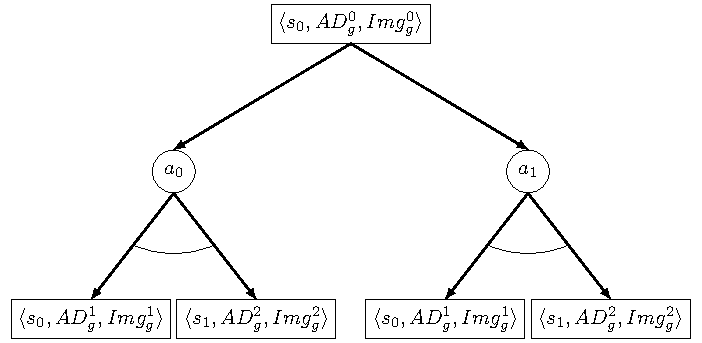
\includegraphics{images/MasterThesisRepNetTreeDraw.pdf}
  \end{center}
  \caption{Look-ahead search space, depth $D=1$ (RepNet-MDP)}\label{fig:repnettree}
\end{figure}

After constructing the search space, an estimation of the value function needs to be back-propagated from the leaves to the root of the tree. An \textit{admissible} heuristic estimate of the true value function
\begin{align}
    h : \Theta_g \rightarrow \R
\end{align}
can be computed at the leaves by taking the base case of the Bellman equations for RepNet-MDPs:
\begin{align}
    h(\theta_g) = \max_{a \in \mathcal{A}} \Big\{ PI_g(s,AD_g,a) \Big\}.
\end{align}
The \textit{epistemic state-action} values are then computed at the action nodes as follows:
\begin{align}
     q(\theta_g, a) = PI_g(s,AD_g,a) + \gamma \sum_{s' \in \mathcal{S}} T_g(g,s,a,s',r_g) h(\big \langle s', \phi_g' \big \rangle).
\end{align}
Non-leaf state nodes use the maximum of the \textit{epistemic state-action} values of their children as their estimate of the value function, i.e.
\begin{align}
    h(\theta_g) = \max_{a \in \mathcal{A}} \Big\{ q(\theta_g, a)  \Big\}.
\end{align}

\section{General discussion: the reputation on a conceptual level}
\label{sec:genn}

The present section briefly discusses the current definition of reputation on a conceptual level and serves as a comment on how it might have to be revised in future work. 

The current definition of reputation (\RefDef{def:repnew}), while arguably intuitive, can lead to undesirable results in regards to self-reputation, fault of its simplicity. This is best demonstrated with an example. Let $A$ and $B$ be two agents, and $Img_A$ agent $A$'s image function, such that:

\begin{align}
    Img_A(B, A) = -1, \,\,\,\,\,\,\,\, Img_A(B,A) = -1,
\end{align}
meaning that in agent $A$'s eyes, $B$ has a poor image of $A$, and $A$ has a poor image of $B$. By definition of the image function, $Img_A(i,i) = 1 \,\,\,\, \forall i \in \mathcal{G}$. As such the self-reputation of agent $A$ is given by:

\begin{align*}
\label{eq:selfrep}
    REP_A(A, Img_A) &= \frac{1}{2} \,\, \big[ Img_A(A,B) \times Img_A(B,A) + Img_A(A,A) \times Img_A(A,A) \big]
    \\&= \frac{1}{2} \,\, \big[ 1 + 1\big] = 1
\end{align*}

Agent $A$ believes its own reputation to be good, despite the fact that it thinks $B$ has a poor image of $A$. Given that $A$ and $B$ are the only agents in the network, this skewed perception of its own reputation could result in agent $A$ performing sub-optimal actions in the network.
